\chapter{Global analysis of the human transcriptome}\label{ch:atlases}

\begin{quotation}
\emph{When we try to pick out anything by itself, we find that it is bound fast by a thousand invisible cords that cannot be broken, to everything in the universe.}
\begin{flushright}
%\citep{Muir1869}
J. Muir (1869)
\end{flushright}
\end{quotation}


Measurements of transcriptional activity provide only a partial view
to physiological processes, but their wide availability provides a
unique resource for investigating gene activity at a genome- and
organism-wide scale. Versatile and carefully controlled {\it gene
expression atlases} have become available for normal human tissues,
cancer as well as for other diseases \citep[see, for
instance,][]{Kilpinen08, Lukk10, Roth06, Su04}. These data sources
contain valuable information about shared and unique mechanisms
between disparate conditions, which is not available in smaller and
more specific experiments \citep{Lage08, Scherf2000}.  While standard
methods for gene expression analysis have focused on comparisons
between particular conditions, versatile transcriptome atlases allow
for global organism-wide characterization of transcriptional
activation patterns \citep{Levine06}. Novel methodological approaches
are needed in order to realize the full potential of these information
sources, as many traditional methods for expression analysis are not
applicable to versatile large-scale collections. This chapter provides
an overview to current approaches for global transcriptome analysis in
Section~\ref{sec:standard} and introduces the second main contribution
of the thesis, a novel exploratory approach that can be used to
investigate context-specific responses in genome-scale interaction
networks across organism-wide collections of measurement data in
Section~\ref{sec:atlas}. The conclusions are summarized in
Section~\ref{sec:atlasconclusion}. 



\section{Standard approaches}\label{sec:standard}

Global observations of transcriptional activity reflect known and
previously uncharacterized cell-biological processes. Exploratory
analysis of the transcriptome can provide research hypotheses and
material for more detailed investigations. Widely-used standard
approaches for global transcriptome analysis include various
clustering, dimensionality reduction and visualization techniques
\citep[see e.g.][]{Huttenhower2010, Polanski07, Quackenbush01}.  The
large data collections open up new possibilities to investigate
functional relatedness between physiological conditions, disease
states, as well as cellular processes, and to discover previously
uncharacterized connections and functional mechanisms
\citep{Bergmann04, Kilpinen08, Lukk10}.

Gene expression studies have traditionally focused on the analysis of
relatively small and targeted data sets, such as particular diseases
or cell types. A typical objective is to detect genes, or gene groups,
that are differentially expressed between particular conditions, for
instance to predict disease outcomes, or to identify potentially
unknown disease subtypes.  The increasing availability of large and
versatile transcriptome collections that may cover thousands of
experimental conditions allows global, data-driven analysis, and the
formulation of novel research questions where the traditional analysis
methods are often insufficient \citep{Huttenhower2010}.  

A variety of approaches have been proposed and investigated in the
recent years in the global transcriptome analysis context. An actively
studied modeling problem in transcriptome analysis is the {\it
  discovery of transcriptional modules}, i.e., identification of
coherent gene groups that show coordinated transcriptional responses
under particular conditions \citep{Segal03psb, Segal04nature,
  Stuart03}. Models have also been proposed to predict gene regulators
\citep{Segal03nature}, and to infer cellular processes and networks
based on transcriptional activation patterns \citep{Friedman04,
  Segal03a}. An increasing number of models are being developed to
integrate transcriptome measurements to other sources of genomic
information, such as regulation and interactions between the genes to
detect and characterize cellular processes and disease mechanisms
\citep{Barash02, Chari2010a, Vaske2010}.  Findings from transcriptome
analysis have potential biomedical implications, as in \cite{Lamb06},
where chemically perturbed cancer cell lines were screened to enhance
the detection of drug targets based on shared functional mechanisms
between disparate conditions, or in \cite{Sorlie01}, where cluster
analysis of cancer patients based on genome-wide transcriptional
profiling experiments led to the discovery of a novel breast cancer
subtype. In the remainder of this section, the modeling approaches
that are particularly closely related to the contributions of this
thesis are considered in more detail.


\subsubsection{Investigating known processes}

A popular strategy for genome-wide gene expression analysis is to
consider known biological processes and their activation patterns
across diverse collections measurement data from various experimental
conditions.  Biomedical databases contain a variety of information
concerning genes and their interactions. For instance, the Gene
Ontology database \citep{Ashburner00} provides functional and
molecular classifications for the genes in human and a number of other
organisms. Other categories are based on micro-RNA regulation,
chromosomal locations, chemical perturbations and other features
\citep{Subramanian05}. Joint analysis of functionally related genes
can increase the statistical power of the analysis.  So-called {\it
  gene set-based approaches} are typically designed to test
differential expression between two particular conditions
\citep{Goeman07, Nam08}, but they can also be used to build global
maps of transcriptional activity of the known processes
\citep{Levine06}. However, gene set-based approaches typically ignore
more detailed information of the interactions between individual
genes. Pathway and interaction databases contain more detailed
information concerning molecular interactions and cell-biological
processes \citep{Kanehisa08, Vastrik07}.  {\it Network-based methods}
utilize relational information of the genes to guide expression
analysis. For instance, \cite{Draghici07} demonstrated that taking
into account aspects of pathway topology, such as gene and interaction
types, can improve the estimation of pathway activity between two
predefined conditions. Another recent approach which utilizes pathway
topology in inferring pathway activity is PARADIGM \citep{Vaske2010},
which also integrates other sources of genomic information in pathway
analysis. However, these methods have been designed for the analysis
of particular experimental conditions, rather than comprehensive
expression atlases. MATISSE \citep{Ulitsky07} is a network-based
approach that searches for functionally related genes that are
connected in the network, and have correlated expression profiles
across many conditions. The potential shortcoming of this approach is
that it assumes global correlation across all conditions between the
interacting genes, while many genes can have multiple,
context-sensitive functional roles.  Different conditions induce
different responses in the same genes, and the definition of 'gene
set' is vague \citep{Montaner09, Nacu07}. Therefore methods have been
suggested to identify 'key condition-responsive genes' of predefined
gene sets \citep{Lee08c}, or to decompose predefined pathways into
smaller and more specific functional modules \citep{Chang09}. These
approaches rely on predefined functional classifications for the
genes. The data-driven analysis in Publication~\ref{NR} provides a
complementary approach where the gene sets are learned directly from
the data, guided by prior knowledge of genetic interactions. This
avoids the need to refine suboptimal annotations, and enables the
discovery of new processes. The findings demonstrate that simply
measuring whether a gene set, or a network, is differentially
expressed between particular conditions is often not sufficient for
measuring the activity of cell-biological processes. Since gene
function and interactions are regulated in a context-specific manner,
it is important to additionally characterize how, and in which
conditions the expression changes. Global analysis of transcriptional
activation patterns interaction networks, introduced in
Publication~\ref{NR}, can address such questions.


\subsubsection{Biclustering and subspace clustering}

Approaches that are based on previously characterized genes and
processes are biased towards well-characterized phenomena. This limits
their value in {\it de novo} discovery of functional patterns.
Unsupervised methods provide tools for such analysis, but often with
an increased computational cost and a higher proportion of false
positive findings.

{\it Cluster analysis} is widely used for unsupervised analysis of
gene expression data, providing tools for class discovery, gene
function prediction and for visualization purposes. Examples of widely
used clustering approaches include hierarchical clustering and K-means
\citep[see e.g.][]{Polanski07}. Clustering of patient samples with
similar expression profiles has led to the discovery of novel cancer
subtypes with biomedical implications \citep{Sorlie01}; clustering of
genes with coordinated activation patterns can be used, for instance,
to predict novel functional associations for poorly characterized
genes \citep{Allocco04}. The self-organizing map \citep{Kohonen82,
  Kohonen01} is a related approach that provides efficient tools to
{\it visualize} high-dimensional data on lower-dimensional displays,
with particular applications in transcriptional profiling studies
\citep{Tamayo99, Toronen99}.  The standard clustering methods are
based on comparison of global expression patterns, and therefore are
relatively coarse tools for analyzing large transcriptome collections.
Different genes respond in different ways, as well as in different
conditions.  Therefore it is problematic to find clusters in
high-dimensional data spaces, such as in whole-genome expression
profiling studies; different gene groups can reveal different
relationships between the samples. Detection of smaller, coherent
subspaces with a particular structure can be useful in biomedical applications, 
where the objective is to identify sets of interesting genes for further analysis. 
Both genes and the associated conditions may be unknown, and
the learning task is to detect them from the data. This can help, for
instance, in identifying responses to drug treatments in particular genes
\citep{Ihmels02, Tanay02bioinf}, or in identifying functionally coherent
transcriptional modules in gene expression databases
\citep{Segal04nature, Tanay05msb}.

{\it Subspace clustering} methods \citep{Parsons04} provide a family
of algorithms that can be used to identify subsets of dependent
features revealing coherent clustering for the samples; this defines a
subspace in the original feature space. Subspace clustering models are
a special case of a more general family of {\it biclustering}
algorithms \citep{Madeira04}. Closely related models are also called
co-clustering \citep{Cho04}, two-way clustering \citet{Getz00}, and
plaid models \citep{Lazzeroni02}. Biclustering methods provide general
tools to detect co-regulated gene groups and associated conditions
from the data, to provide compact summaries and to aid interpretation
of transcriptome data collections. Biclustering models enable the
discovery of {\it gene expression signatures} \citep{Hu06} that have
emerged as a central concept in global expression analysis context. A
signature describes a co-expression state of the genes, associated
with particular conditions. Established signatures have been found to
be reliable indicators of the physiological state of a cell, and
commercial signatures have become available for routine clinical
practice \citep{Nuyten08}. However, the established signatures are
typically designed to provide optimal classification performance
between two particular conditions. The problem with the
classification-based signatures is that their associations to the
underlying physiological processes are not well understood
\citep{Lucas09}. In Publication~\ref{NR} the understanding is enhanced
by deriving transcriptional signatures that are explicitly connected
to well-characterized processes through the network.

\subsubsection{Role of side information}

Standard clustering models ignore prior information of the data, which
could be used to supervise the analysis, to connect the findings to
known processes, as well as to improve scalability. For instance,
standard model-based feature selection, or subspace clustering
techniques would consider all potential connections between the genes
or features \citep{Law04, Roth04}. Without additional constraints on
the solution space they can typically handle at most tens or hundreds
of features, which is often insufficient in high-throughput genomics
applications.  Use of side information in clustering can help to guide
unsupervised analysis, for instance based on known or potential
interactions between the genes. This has been shown to improve the
detection of functionally coherent gene groups \citep{Hanisch02,
Shiga07, Ulitsky07, Zhu05}. However, while these methods provide tools
to cluster the genes, they do not model differences between
conditions. Extensions of biclustering models that can utilize
relational information of the genes include cMonkey \citep{Reiss06}
and a modified version of SAMBA biclustering \citep{Tanay04}. However,
cMonkey and SAMBA are application-oriented tools that rely on
additional, organism-specific information, and their implementation is
currently not available for most organisms, including that of the
human.  Further application-oriented models for utilizing side
information in the discovery of transcriptional modules have recently
been proposed for instance by \cite{Savage2010} and \cite{Suthram10}.
Publication~\ref{NR} introduces a complementary method where the
exhaustively large search space is limited with side information
concerning known relations between the genes, derived from genomic
interaction databases. This is a general algorithmic approach whose
applicability is not limited to particular organisms.

\subsubsection{Other approaches}

Prior information on the cellular networks, regulatory mechanisms, and
gene function is often available, and can help to construct more
detailed models of gene function and network analysis, as well as to
summarize functional aspects of genomic data collections
\citep{Huttenhower09, Segal03nature, Troyanskaya05}. Versatile
transcriptome collections also enable {\it network reconstruction},
i.e., {\it de novo} discovery \citep{Lezon06, Myers05} and
augmentation \citep{Novak06} of genetic interaction networks. Other
methodological approaches for global transcriptome analysis are
provided by probabilistic latent variable models \citep{Rogers05,
  Segal03psb}, hierarchical Dirichlet process algorithms
\citep{Gerber07}, as well as matrix and tensor computations
\citep{Alter05}. These methods provide further model-based tools to
identify and characterize transcriptional programs by decomposing gene
expression data sets into smaller, functionally coherent components.


\section{Global modeling of transcriptional activity in interaction
  networks}\label{sec:atlas}


Molecular interaction networks cover thousands of genes, proteins and
small molecules. Coordinated regulation of gene function through
molecular interactions determines cell function, and is reflected in
transcriptional activity of the genes.  Since individual processes and
their transcriptional responses are in general unknown \citep{Lee08c,
  Montaner09}, data-driven detection of condition-specific responses
can provide an efficient proxy for identifying distinct
transcriptional states of the network with potentially distinct
functional roles. While a number of methods have been proposed to
compare network activation patterns between particular conditions
\citep{Draghici07, Ideker02, Cabusora05, Noirel08}, or to use network
information to detect functionally related gene groups
\citep{Segal03b, Shiga07, Ulitsky07}, general-purpose algorithms for a
global analysis of context-specific network activation patterns in a
genome- and organism-wide scale have been missing.

Publication~\ref{NR} introduces and validates two general-purpose
algorithms that provide tools for global modeling of transcriptional
responses in interaction networks. The motivation is similar to
biclustering approaches that detect functionally coherent gene groups
that show coordinated response in a subset of conditions
\citep{Madeira04}. The network ties the findings more tightly to
cell-biological processes, focusing the analysis and improving
interpretability. In contrast to previous network-based biclustering
models for global transcriptome analysis, such as cMonkey
\citep{Reiss06} or SAMBA \citep{Tanay04}, the algorithms introduced in
Publication~\ref{NR} are general-purpose tools, and do not depend on
organism-specific annotations.


\subsubsection{A two-step approach}

The first approach in Publication~\ref{NR} is a straightforward
extension of network-based gene clustering methods. In this two-step
approach, the functionally coherent subnetworks, and their
condition-specific responses are detected in separate steps. In the
first step, a network-based clustering method is used to detect
functionally coherent subnetworks.  In Publication~\ref{NR}, MATISSE,
a state-of-the-art algorithm described in \cite{Ulitsky07}, is used to
detect the subnetworks. MATISSE finds connected subgraphs in the
network that have high internal correlations between the genes.  In
the second step, condition-specific responses of each identified
subnetwork are searched for by a nonparametric Gaussian mixture model,
which allows a data-driven detection of the responses. However, the
two-step approach, coined MATISSE+, can be suboptimal for detecting
subnetworks with particular condition-specific responses. The main
contribution of Publication~\ref{NR} is to introduce a second
general-purpose algorithm, coined NetResponse, where the detection of
condition-specific responses is used as the explicit key criterion for
subnetwork search.

\begin{figure}[t]
\begin{center}
\centering{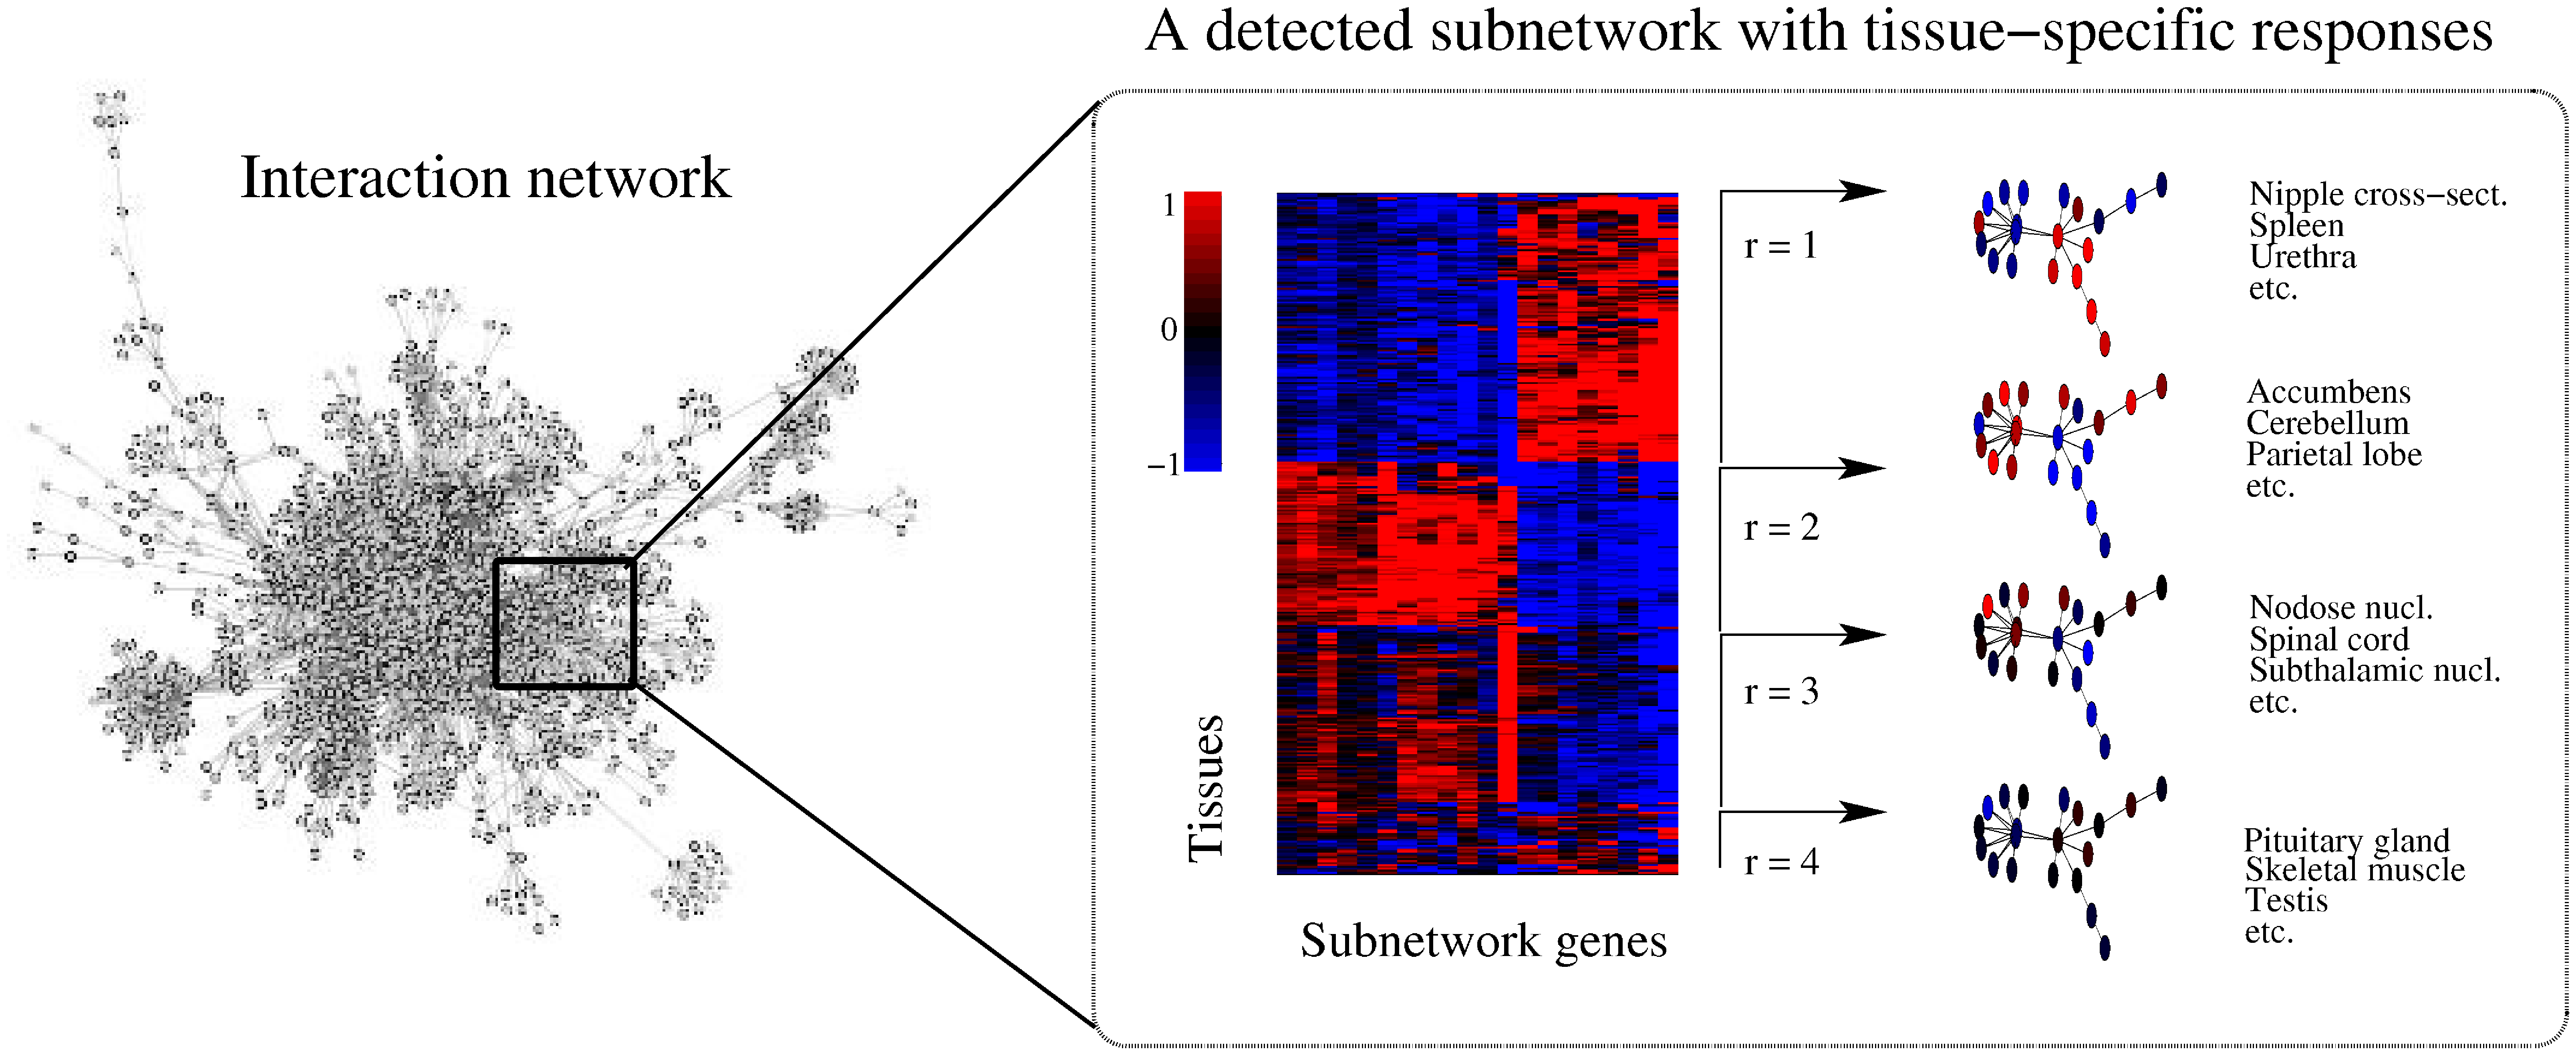
\includegraphics[width=\textwidth]{pic/methodVertical6cropped.eps}}
\end{center}
\caption{Organism-wide analysis of transcriptional responses in a
  human pathway interaction network reveals physiologically coherent
  activation patterns and condition-specific regulation. One of the
  subnetworks and its condition-specific responses, as detected by the
  NetResponse algorithm is shown in the Figure. The expression of each
  gene is visualized with respect to its mean level of expression
  across all samples. \copyright The Author 2010. Published by Oxford
  University Press. Reprinted with permission from
  Publication~\ref{NR}.}
\label{fig:netresponse}
\end{figure}

\subsubsection{The NetResponse algorithm}\label{sec:netresponse}

The network-based search procedure introduced in Publication~\ref{NR}
searches for local {\it subnetworks}, i.e., functionally coherent
network modules where the interacting genes show coordinated responses
in a subset of conditions (Figure~\ref{fig:netresponse}).  Side
information of the gene interactions is used to guide modeling, but
the algorithm is independent of predefined classifications for genes
or measurement conditions. Transcriptional responses of the network
are described in terms of subnetwork activation. Regulation of the
subnetwork genes can involve simultaneous activation and repression of
the genes: sufficient amounts of mRNA for key proteins has to be
available while interfering genes may need to be silenced. The model
assumes that a given subnetwork \(n\) can have multiple
transcriptional states, associated with different physiological
contexts. A transcriptional state is reflected in a unique expression
signature \(\s^{(n)}\), a vector that describes the expression levels
of the subnetwork genes, associated with the particular
transcriptional state. Expression of some genes is regulated at
precise levels, whereas other genes fluctuate more freely. Given the
state, expression of the subnetwork genes is modeled as a noisy
observation of the transcriptional state. With a Gaussian noise model
with covariance \(\Sigma^{(n)}\), the observation is described by
\(\xn \sim N(\s^{(n)}, \Sigma^{(n)})\). A given subnetwork can have
\(\Rn\) latent transcriptional states indexed by \(r\).  In practice,
the states, including their number \(\Rn\), are unknown, and they have
to be estimated from the data.  In a specific measurement condition,
the subnetwork $n$ can be in any one of the latent physiological
states indexed by $r$. Associations between the observations and the
underlying transcriptional states are unknown and they are treated as
latent variables. Gene expression in subnetwork \(n\) is then modeled
with a Gaussian mixture model:

\begin{equation}
  \xn \sim \sum_{r=1}^{\Rn} \wrn p(\xn | \bth_r ),
  \label{eq:gm}
\end{equation}

\noindent where each component distribution $p$ is assumed to be
Gaussian with parameters \(\bth_r = \{\srn, \Sigrn\}\).  In practice,
we assume a diagonal covariance matrix \(\Sigrn\), leaving the
dependencies between the genes unmodeled within each transcriptional
state. Use of diagonal covariances is justified by considerable gains
in computational efficiency when the detection of distinct responses
is of primary interest. It is possible, however, that such simplified
model will fail to detect certain subnetworks where the
transcriptional levels of the genes have strong linear dependencies
within the individual transcriptional states; signaling cascades
could be expected to manifest such activation patterns, for
instance. More detailed models of transcriptional activity could help
to distinguish the individual states in particular when the
transcriptional states are partially overlapping, but with increased
computational cost. A particular transcriptional response is then
characterized with the triple \(\{\srn, \Sigrn, \wrn\}\). This defines
the shape, fluctuations and frequency of the associated
transcriptional state of subnetwork \(n\).  A posterior probability of
each latent state can be calculated for each measurement sample from
the Bayes' rule (Equation~\ref{eq:bayesrule}). The posterior
probabilities can be interpreted as soft component memberships for the
samples. A hard, deterministic assignment is obtained by selecting for
each sample the component with the highest posterior probability.

The remaining task is to identify the subnetworks having such distinct
transcriptional states. Detection of the distinct states is now used
as a search criterion for the subnetworks. In order to achieve fast
computation, an agglomerative procedure is used where interacting
genes are gradually merged into larger subnetworks.  Initially, each
gene is assigned in its own singleton subnetwork. Agglomeration
proceeds by at each step merging the two neighboring subnetworks where
joint modeling of the genes leads to the highest improvement in the
objective function value. Joint modeling of dependent genes reveals
coordinated responses and improves the likelihood of the data in
comparison with independent models, giving the first criterion for
merging the subnetworks. However, increasing subnetwork size tends to
increase model complexity and the possibility of overfitting, since
the number of samples remains constant while the dimensionality
(subnetwork size) increases. To compensate for this effect, the
Bayesian information criterion \citep[see][]{Gelman03} is used to
penalize increasing model complexity and to determine optimal
subnetwork size. The final cost function for a subnetwork \(G\) is
\(C(G) = - 2\L + q log(N)\), where \(\L\) is the (marginal)
log-likelihood of the data, given the mixture model in
Equation~\ref{eq:gm}, \(q\) is the number of parameters and \(N\) denotes
sample size. The algorithm then compares independent and joint models
for each subnetwork pair that has a direct link in the network, and
merges at each step the subnetwork pair \(G_i, G_j\) that minimizes
the cost

\begin{equation}\label{eq:netreponsecost}
  \Delta\mathcal{C} = - 2(\L_{i,j} - (\L_i + \L_j)) + (q_{i,j} - (q_i + q_j))log(N). 
\end{equation}

The iteration continues until no improvement is obtained by merging
the subnetworks. The combination of modeling techniques yields a
scalable algorithm for genome- and organism-wide investigations:
First, the analysis focuses on those parts of the data that are
supported by known interactions, which increases modeling power and
considerably limits the search space. Second, the agglomerative scheme
finds a fast approximative solution where at each step the subnetwork
pair that leads to the highest improvement in cost function is
merged. Third, an efficient variational approximation is used to learn
the mixture models \citep{Kurihara07nips}. Note that the algorithm
does not necessarily identify a globally optimal solution. However,
detection of physiologically coherent and reproducible responses is
often sufficient for practical applications.

\subsubsection{Global view on network activation patterns}

The NetResponse algorithm introduced in Publication~\ref{NR} was
applied to investigate transcriptional activation patterns of a
pathway interaction network of 1800 genes based on the KEGG database
of metabolic pathways \citep{Kanehisa08} provided by the SPIA package
\citep{Tarca09} across 353 gene expression samples from 65
tissues. The two algorithms proposed in Publication~\ref{NR}, MATISSE+
and NetResponse were shown to outperform an unsupervised biclustering
approach in terms of reproducibility of the finding. The introduced
NetReponse algorithm, where the detection of transcriptional response
patterns is used as a search criterion for subnetwork identification,
was the best-performing method. The algorithm identified 106
subnetworks with 3-20 genes, with distinct transcriptional responses
across the conditions. One of the subnetworks is illustrated in
Figure~\ref{fig:netresponse}; the other findings are provided in the
supplementary material of Publication~\ref{NR}. The detected
transcriptional responses were physiologically coherent, suggesting a
potential functional role. The reproducibility of the responses was
confirmed in an independent validation data set, where 80\% of the
predicted responses were detected (\(p < 0.05\)). The findings
highlight context-specific regulation of the genes.  Some responses
are shared by many conditions, while others are more specific to
particular contexts such as the immune system, muscles, or the brain;
related physiological conditions often exhibit similar network
activation patterns. Tissue relatedness can be measured in terms of
shared transcriptional responses of the subnetworks, giving an
alternative formulation of the tissue connectome map suggested by
\cite{Greco08} in order to highlight functional connectivity between
tissues based on the number of shared differentially expressed genes.
In Publication~\ref{NR}, shared network responses are used instead of
shared gene count. The use of co-regulated gene groups is expected to
be more robust to noise than the use of individual genes.  The
analysis provides a global view on network activation across the
normal human body, and can be used to formulate novel hypotheses of
gene function in previously unexplored contexts.

\section{Conclusion}\label{sec:atlasconclusion}

Gene function and interactions are often subject to condition-specific
regulation \citep{Liang06, Rachlin06}, but these have been typically
studied only in particular experimental conditions. Organism-wide
analysis can potentially reveal new functional connections and help to
formulate novel hypotheses of gene function in previously unexplored
contexts, and to detect highly specialized functions that are specific
to few conditions. Changes in cell-biological conditions induce
changes in the expression levels of co-regulated genes, in order to
produce specific physiological responses, typically affecting only a
small part of the network. Since individual processes and their
transcriptional responses are in general unknown \citep{Lee08c,
  Montaner09}, data-driven detection of condition-specific responses
can provide an efficient proxy for identifying distinct
transcriptional states of the network, with potentially distinct
functional roles.

Publication~\ref{NR} provides efficient model-based tools for global,
organism-wide discovery and characterization of context-specific
transcriptional activity in genome-scale interaction networks,
independently of predefined classifications for genes and
conditions. The network is used to bring in prior information of gene
function, which would be missing in unsupervised models, and allows
data-driven detection of coordinately regulated gene sets and their
context-specific responses. The algorithm is readily applicable in any
organism where gene expression and pairwise interaction data,
including pathways, protein interactions and regulatory networks, are
available. It has therefore a considerably larger scope than previous
network-based models for global transcriptome analysis, which rely on
organism-specific annotations, but lack implementations for most
organisms \citep{Reiss06, Tanay04}.

While biomedical implications of the findings require further
investigation, the results highlight shared and reproducible responses
between physiological conditions, and provide a global view of
transcriptional activation patterns across the normal human
body. Other potential applications for the method include large-scale
screening of drug responses and disease subtype
discovery. Implementation of the algorithm is freely available through
BioConductor.\footnote{http://bioconductor.org/packages/devel/bioc/html/netresponse.html}


